\documentclass{beamer}
\beamertemplatenavigationsymbolsempty 

\title{Detecting Asteroids with Neural Networks}
\author{Dustin Ingram}
\institute{Advanced Artificial Intelligence, Winter 12-13\\ Drexel University
Department of Computer Science}
\date{\today}

\begin{document}
\maketitle

\begin{frame}
    \frametitle{Outline}
    \begin{itemize}
        \item What's the goal?
        \item What's the data?
        \item Getting started
        \item Building a feature set
        \item Building the neural network
        \item Training the network
        \item Results
    \end{itemize}
\end{frame}

\begin{frame}
    \frametitle{The goal}
    Build and train a neural network to correctly identify asteroids in
    astrophotography data.
\end{frame}

\begin{frame}
    \frametitle{So...}
    How do we do it?
\end{frame}

\begin{frame}
    \frametitle{So...}
    How do we \emph{really} do it?
\end{frame}

\begin{frame}
    \frametitle{The data}
    The Sloan Digital Sky Survey:
    \begin{itemize}
        \item "One of the most ambitious and influential surveys in the history
        of astronomy."
        \item Approx 35\% of sky
        \item Largest uniform survey of the sky yet accomplished
        \item Data is freely available online
        \item Each image is 922x680 pixels
    \end{itemize}
\end{frame}

{
    \usebackgroundtemplate{\includegraphics[width=\paperwidth,height=\paperheight]{18364_unbox.jpg}}
    \begin{frame}[plain] \end{frame}
}

{
    \usebackgroundtemplate{\includegraphics[width=\paperwidth,height=\paperheight]{18364_box.png}}
    \begin{frame}[plain] \end{frame}
}

\begin{frame}
    \frametitle{An example asteroid}
    \begin{figure}
        \centering
        \includegraphics{18364.jpg}
    \end{figure}
\end{frame}

\begin{frame}
    \frametitle{An example asteroid}
    \begin{figure}
        \centering
        \includegraphics[height=0.8\paperheight]{18364_large.jpg}
    \end{figure}
\end{frame}

\begin{frame}
    \frametitle{How does this work?}
    This exploits a property of CCDs:
    \begin{itemize}
        \item SDSS telescopes use five different filters
        \item They are not simultaneous
        \item Moving objects appear in different locations
        \item Always the same order
    \end{itemize}
\end{frame}

\begin{frame}
    \frametitle{An example asteroid}
    \begin{figure}
        \centering
        \includegraphics[height=0.8\paperheight]{18364_large.jpg}
    \end{figure}
\end{frame}

\begin{frame}
    \frametitle{Getting started}
    Getting the initial training data:
    \begin{itemize}
        \item Small tool to extract potential candidates from full-scale images
        \item Extremely na\"{\i}ve, approx 100:5 false positives to actual positives
        \item Very low false negatives (approx 1:1000)
        \item Incredibly slow (complex scan of 100Ks of potentials)
        \item Manual classification, somewhat slow
        \item Yields approx 250 valid items, 500 invalid items
    \end{itemize}
\end{frame}

%\begin{frame}
%    \frametitle{The feature set}
%    Bad ideas for features:
%    \begin{itemize}
%        \item Average ``high'' and ``low'' values ($v > 0.5$, $v < 0.5$)
%        \item Ratio of ``high'' to all colored ($0.25 < v < 0.4$)
%        \item Ratio of ``low'' to all colored ($0.6 < v < 0.75$)
%        \item Ratio of ``invalid'' to all colored ($0.4 < v < 0.6$)
%    \end{itemize}
%\end{frame}

\begin{frame}
    \frametitle{The feature set}
    Good ideas for features:
    \begin{itemize}
        \item Ratio valid hues to non-valid hues
        \item Best possible cluster collinearity
        \item Best possible average cluster distance
    \end{itemize}
\end{frame}

\begin{frame}
    \frametitle{Feature: Ratio valid hues to non-valid hues}
    The goal here is to match the colors, a.k.a. ``hues'':
    \begin{itemize}
        \item First step: convert to HSV space
        \item For pixels in the valid value-spectrum ($0.25 < v < 0.90$)
        \item How many are within 2 standard deviations from an optimal value?
        \item What's the ratio to ones that aren't?
    \end{itemize}
\end{frame}

\begin{frame}
    \frametitle{An example HSV plot}
    \begin{figure}
        \centering
        \includegraphics[width=0.85\paperwidth]{chart_1.png}
    \end{figure}
\end{frame}

\begin{frame}
    \frametitle{Feature: Best possible cluster collinearity}
    $k$-means clustering
    \begin{itemize}
        \item Using the valid hues from the previous feature
        \item Attempts to cluster $n$ points into $k$ groups
        \item Here, $k=3$
        \item Produces three centroids
    \end{itemize}
\end{frame}

\begin{frame}
    \frametitle{An example asteroid}
    \begin{figure}
        \centering
        \includegraphics[height=0.8\paperheight]{18364_large.jpg}
    \end{figure}
\end{frame}

\begin{frame}
    \frametitle{$k$-means clustering of the same asteroid}
    \begin{figure}
        \centering
        \includegraphics[height=0.8\paperheight]{clust-18364.png}
    \end{figure}
\end{frame}

\begin{frame}
    \frametitle{Feature: Best possible cluster collinearity}
    Collinearity:
    \begin{itemize}
        \item The property of a set of points which lie on the same line
        \item Iterate the $k$-means clustering approx. 20 times
        \item The resulting metric is the ratio between the actual collinearity
        and the maximum potential colinearity
        \item Given points $a$, $b$, and $c$:
    \end{itemize}

        \begin{equation*}
            colin = | (c.x - a.x) * (b.y - a.y) + (c.y - a.y) * (a.x - b.x) |
        \end{equation*}
\end{frame}

\begin{frame}
    \frametitle{An example asteroid}
    \begin{figure}
        \centering
        \includegraphics[height=0.8\paperheight]{18364_large.jpg}
    \end{figure}
\end{frame}

\begin{frame}
    \frametitle{$k$-means clustering of the same asteroid}
    \begin{figure}
        \centering
        \includegraphics[height=0.8\paperheight]{clust-18364.png}
    \end{figure}
\end{frame}

\begin{frame}
    \frametitle{An example non-asteroid}
    \begin{figure}
        \centering
        \includegraphics[height=0.8\paperheight]{494_large.jpg}
    \end{figure}
\end{frame}

\begin{frame}
    \frametitle{$k$-means clustering of the same non-asteroid}
    \begin{figure}
        \centering
        \includegraphics[height=0.8\paperheight]{clust-494.png}
    \end{figure}
\end{frame}

\begin{frame}
    \frametitle{Feature: Best possible average cluster distance}
    \begin{itemize}
        \item Using the same $k$-means clusters from the previous features
        \item What is the average distance from any point in a cluster to the
        center of the cluster?
    \end{itemize}
\end{frame}

\begin{frame}
    \frametitle{An example asteroid}
    \begin{figure}
        \centering
        \includegraphics[height=0.8\paperheight]{18364_large.jpg}
    \end{figure}
\end{frame}

\begin{frame}
    \frametitle{$k$-means clustering of the same asteroid}
    \begin{figure}
        \centering
        \includegraphics[height=0.8\paperheight]{clust-18364.png}
    \end{figure}
\end{frame}

\begin{frame}
    \frametitle{An example non-asteroid}
    \begin{figure}
        \centering
        \includegraphics[height=0.8\paperheight]{494_large.jpg}
    \end{figure}
\end{frame}

\begin{frame}
    \frametitle{$k$-means clustering of the same non-asteroid}
    \begin{figure}
        \centering
        \includegraphics[height=0.8\paperheight]{clust-494.png}
    \end{figure}
\end{frame}

\begin{frame}
    \frametitle{A comparison of all three features}
    \begin{figure}
    \centering
    \begin{tabular}{|r|c|c|c|}
        \hline
        & \textbf{Hue Ratio} & \textbf{Collinearity} & \textbf{Cluster distance}
        \\\hline
        \textbf{Asteroid} & 0.687 & 0.046 & 0.432\\\hline
        \textbf{Non-asteroid} & 0.376 & 0.388 & 0.557\\\hline
    \end{tabular}
    \end{figure}
    \begin{itemize}
        \item We see that the for a valid asteroid:
        \begin{itemize}
            \item The hue ratio is much higher
            \item The colinearity metric is much lower
            \item The mean cluster disance is smaller
        \end{itemize}
    \end{itemize}
\end{frame}

\begin{frame}
    \frametitle{Ok... where's the AI?}
    This type of classification is extrememly well suited for a neural network:
    \begin{itemize}
        \item We have a clear set of training data
        \item The output is either affirmative (1) or negative (0)
        \item Each of the input features can be resolved to a $0\to 1$ metric
        \item There is a small amount of input features which can accurately
        define an item
        \item Neural network activation will be much faster than almost any
        algorithm we can come up with
    \end{itemize}
\end{frame}

\begin{frame}
    \frametitle{Building the neural network}
    The resulting neural network:
    \begin{itemize}
        \item Use supervised learning
        \item Uses a backpropagation trainer
        \item Three layers:
        \begin{itemize}
            \item Input layer
            \item Single hidden layer
            \item Output layer
        \end{itemize}
        \item Total of 8 ``neurons'':
        \begin{itemize}
            \item 3 input neurons (hue ratio, collinearity metric, distance
            metric)
            \item 4 hidden neurons
            \item 1 output neuron ($1$ if valid asteroid, $0$ if invalid)
        \end{itemize}
        \item Learning rate of $0.01$, momentum of $0.99$
    \end{itemize}
\end{frame}

\begin{frame}
    \frametitle{Building the neural network}
    The resulting neural network:
    \begin{figure}
        \centering
        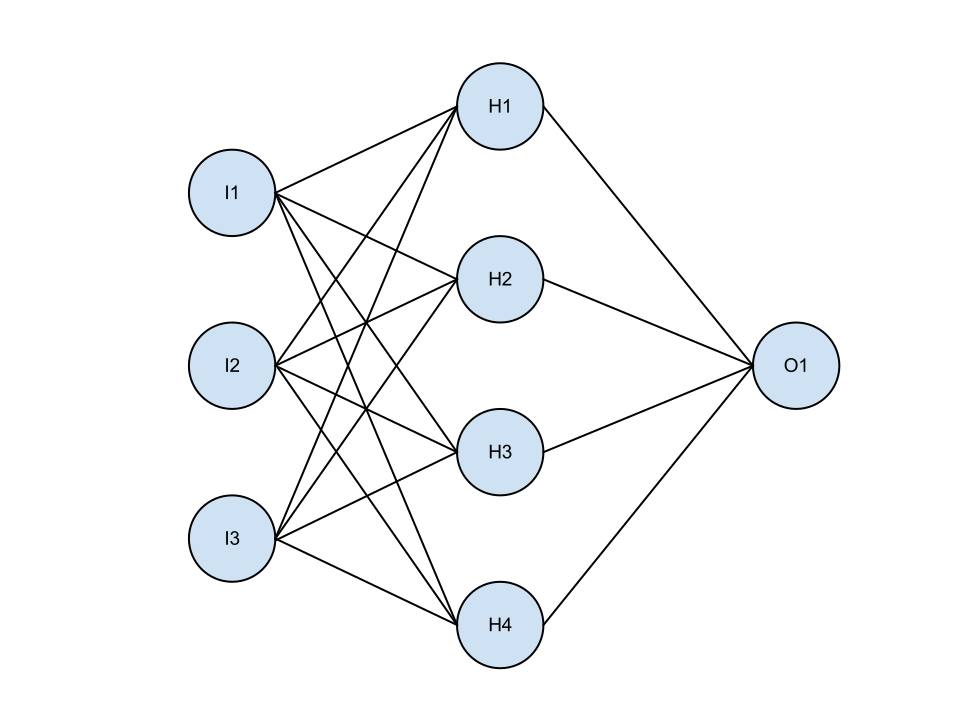
\includegraphics[height=0.8\paperheight]{nn.pdf}
    \end{figure}
\end{frame}

\begin{frame}
    \frametitle{Training the network}
    \begin{itemize}
        \item Approx 250 valid items
        \item Approx 500 invalid items
        \item Trained for 5,000 iterations
        \item Took approx. 3 hours
        \item Probably could have gotten by with less iterations
    \end{itemize}
\end{frame}

\begin{frame}
    \frametitle{Results}
    {\small
    \begin{tabular}{|c|c|c|c|c|c|c|c|}
        \hline
        \textbf{Trial} &  \textbf{Found Valid} & \textbf{Actual Valid} &
        \textbf{Total} & \textbf{False positive} \\\hline
        Trial 1 &   8 &   5 &   190 & 37.50\% \\\hline
        Trial 2 & 23 &  21 &  286 & 8.70\% \\\hline
        Trial 3 & 54 &  46 &  955 & 14.81\% \\\hline
    \end{tabular}
    }
\end{frame}

\begin{frame}
    \frametitle{Results}
    {\small
    \begin{tabular}{|c|c|c|c|c|c|c|c|}
        \hline
        \textbf{Trial} &  \textbf{Found Invalid} & \textbf{Actual Invalid} &
        \textbf{Total} & \textbf{False negative} \\\hline
        Trial 1 & 182 & 182 & 190 & 0.00\% \\\hline
        Trial 2 & 263 & 262 & 286 & 0.38\% \\\hline
        Trial 3 & 901 & 892 & 955 & 1.00\% \\\hline
    \end{tabular}

    }
\end{frame}

\begin{frame}
    \frametitle{Conclusion}
    \begin{itemize}
        \item Using a neural network allows us to do it faster, and more
        accurately
        \item Need to spend time coming up with good features for the data
        \item When paired with human validation, the process would become very
        quick and very accurate

    \end{itemize}
\end{frame}

\begin{frame}
    \frametitle{References}
    \small
    \begin{itemize}
        \item \url{http://www.sdss.org/}
        \item \url{http://pybrain.org/}
        \item \url{http://en.wikipedia.org/wiki/Sloan_Digital_Sky_Survey}
        \item \url{http://en.wikipedia.org/wiki/Collinearity}
        \item \url{http://en.wikipedia.org/wiki/K-means_clustering}
    \end{itemize}
\end{frame}

\end{document}
